\maketitle

\tableofcontents

\section{Introducing Spectral Indices for Vegetation}
Spectral indices or spectral index (singular) is a term used to define a result of mathematical operation (map algebra, raster algebra, etc.) of two or more band of spectrum from a multispectral imagery \cite{xue2017significant}.

 The most famous one of spectral indices is NDVI (Normalized Difference Vegetation Index). It is the result from the margin of near infrared (NIR) and red band divided by the sum of both, following Equation \ref{eq:ndvi}. This index have many use such as to classify certain land cover: soil, built-up, water, sparse, and dense vegetation. It also can be used to monitor vegetation health and pattern over time. The result of NDVI is an image with a value ranging from -1 to 1 where value below 0 tend to be water, 0 to 0.3 is built-up, soil, and grass while above the 0.4 to be shrub and denser vegetation. Although high value can be used to identify if the vegetation is healthy. Example of the multispectral imagery and NDVI can be seen in Figure \ref{fig:imageNdvi}.

\begin{equation}
	\label{eq:ndvi}
	NDVI = \frac{NIR - RED}{NIR + RED}
\end{equation}

\begin{figure}
	\label{fig:imageNdvi}
	\centering
	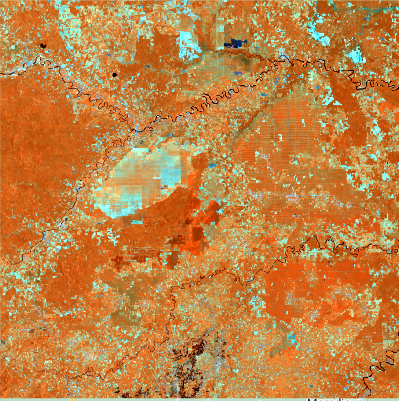
\includegraphics[height=30ex]{komposit.png}
	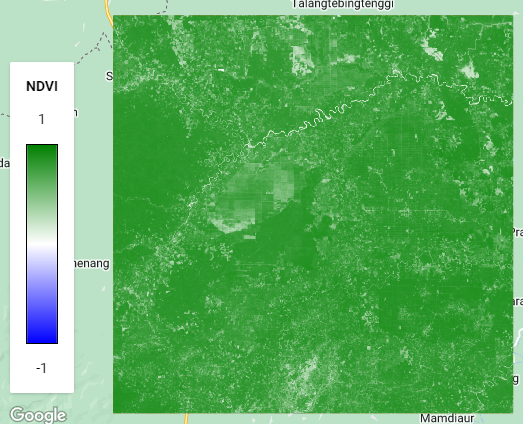
\includegraphics[height=30ex]{ndvi.png}
	\caption{NIR-SWIR1-SWIR2 composite (left) and NDVI (right) image}
\end{figure}

NIR band is used in the formula is following the spectral reflectance curve on how the interaction between multiple electomagnetic wavelength to certain object. This relation could be understand from Figure \ref{fig:spectralCurve}. Based on the curve, it can be understood that the reflectance of vegetation at its peak in NIR band wavelength interval while it have a smaller reflectance in the red spectrum while red band also have a high reflectance in soil object.

\begin{figure}[htbp]
	\label{fig:spectralCurve}
	\centering
	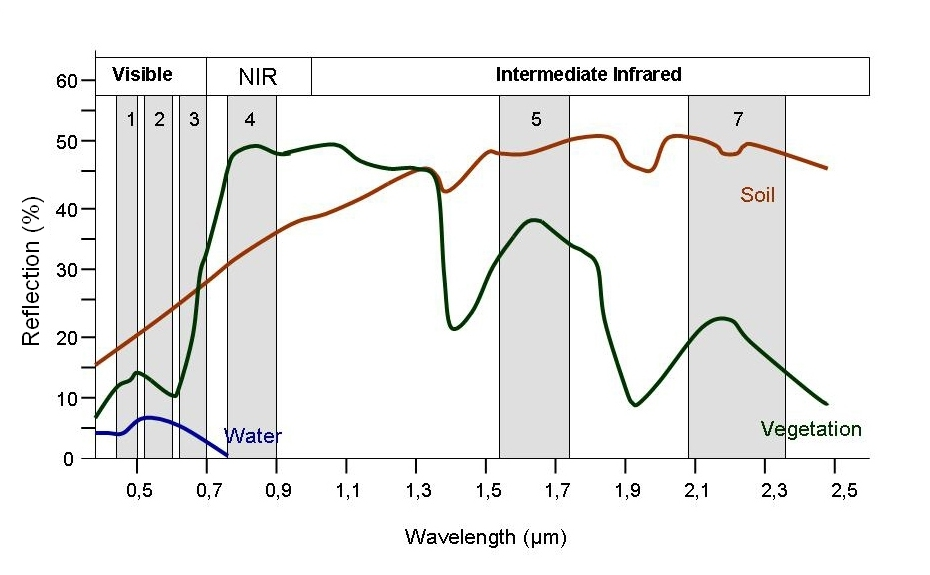
\includegraphics[width=80ex]{Reflexionskurven.jpg}
	\caption{Spectral reflectance curve of soil, vegetation, and water on multiple electromagnetic spectrum \cite{siegmund2005fernes}}
\end{figure}

While NDVI is useful for most cases, it is not perfect for every situation. In highly forested area, NDVI have a hard time to differentiate between more dense canopy. So a new index for vegetation or vegetation indices is developed: Enhanced Vegetation Index (EVI) \cite{huete2002overview}. EVI utlize additional band or spectrum to its calculation. This index while can help on densely forested area, it also able to reduce atmospheric effect. Equation \ref{eq:evi} is used to calculate EVI.

\begin{equation}
	\label{eq:evi}
	EVI = 2.5 * \frac{NIR - RED}{NIR + 6 * RED - 7.5 * BLUE + 1}
\end{equation}

Other than EVI, there are many more vegetation indices for certain purpose and goal. Such as SAVI (Soil-Adjusted Vegetation) where it try to reduce the effect of soil in sparse vegetation \cite{huete1988soil} (Equation \ref{eq:savi}); EMVI (Enhanced Mangrove Vegetation Index) to help identify mangrove vegetation or wet dense vegetation (Equation \ref{eq:emvi}) \cite{yang2022enhanced}; and NBR (Equation \ref{eq:nbr}) (Normalized Burn Ratio) to help analyze burn severity, it can also differenciate between much more dense forest \cite{escuin2008fire}.

\begin{equation}
	\label{eq:savi}
	SAVI = \frac{NIR - RED}{NIR + RED + 0.5} * 1.5
\end{equation}

\begin{equation}
	\label{eq:emvi}
	EMVI = \frac{GREEN - SWIR2}{SWIR1 - GREEN}
\end{equation}

\begin{equation}
	\label{eq:nbr}
	NBR = \frac{NIR - SWIR2}{NIR + SWIR2}
\end{equation}

\section{Calculating Vegetation Indices in Google Earth Engine}
Google Earth Engine (GEE) is cloud-based geospatial analysis software for global scale and multitemporal data \cite{gorelick2017google}. It is allow user to do analysis online without the need for high computation resources. It is also store many remote sensing data that can be use directly. This allow professionals and academics to utilize for many project and research.

Calculating vegetation indices is one method to analyze the landscape using multispectral satellite imagery. This imagery are available in the GEE, so instead of downloading the image then calculate the indices in a GIS software, is it now posibble to do it directly in the cloud. 

In GEE, an imagery or stack of multispectral imagery is represented by \verb|ee.Image| object/class. This object will have several properties such as all the bands of stacked image inside, geometry boundary, date, source, and any other properties. Using the bands available in the \verb|ee.Image|, it is possible to calculate vegetation indices. It could be done using mathematical operation such as \verb|add, subtract, multiply, & divide| or using \verb|ee.Image.expression| method where it receive two arguments: the formula in quoted text/string and band map or the definition of the formula's variables. Script \ref{code:expression} show the example to calculate NDVI using Landsat imagery.

\begin{lstlisting}[language=JavaScript, label={code:expression}, caption={GEE script to calculate NDVI from Landsat 8 OLI imagery}]
// Importing landsat imagery collection surface reflectance (level 2)
var landsat8 = ee.ImageCollection("LANDSAT/LC08/C02/T1_L2");

// ee.Geometry object to filter and clip image
var roi = ee.Geometry({
	"geodesic": false,
	"type": "Polygon",
	"coordinates": [
		[
			[
				102.72375815056746,
				-3.084684226459141
			],
			[
				103.27307455681746,
				-3.084684226459141
			],
			[
				103.27307455681746,
				-2.5387744837647532
			],
			[
				102.72375815056746,
				-2.5387744837647532
			],
			[
				102.72375815056746,
				-3.084684226459141
			]
		]
	]
});

// Filter the imagery using boundary and date
var image = landsat8.filterBounds(roi) // Filter by region
	.filterDate('2023-01-01', '2023-12-31') // Filter by date
	.sort('CLOUD_COVER_LAND') // Sort by the fewest cloud cover
	.first() // Get the first image from the collection
	.clip(roi) // Clip the image
	.select(['SR_B.*'], ['B1', 'B2', 'B3', 'B4', 'B5', 'B6', 'B7']) // Select only useful bands
	.multiply(0.0000275).add(-0.2); // Scaled it to 0-1

// Band map to define the band use for calculation
var bandMap = {
	NIR: image.select('B5'),
	RED: image.select('B4')
};

// Calculate NDVI
var ndvi = image.expression('NDVI = (NIR - RED) / (NIR + RED)', bandMap);

// Show NDVI to map
Map.addLayer(NDVI, { min: -1, max: 1, palette: ['blue', 'white', 'green'] }, 'NDVI');
\end{lstlisting}

\section{Applying Relational Operation to Classify Vegetation Type}
Certain value in vegetation indices could determine the type of land cover or type of vegetation. However, this the values of a certain region might not be fit with other region, so it will always need for assessment per region. Usually, it could be useful to utilize many indices, so not only vegetation, like NDWI (Normalized Difference Water Index) and NDBI (Normalized Difference Built-up Index) to make more diverse classification.

To mask or group certain land cover or vegetation type using indices, you can determine the threshold of the indices value. In GEE, it can utilize using relational operation such as \verb|lt, lte, gt, gte, eq, neq, and, or|, where each will state if our threshold is lower than (\verb|lt|) or greater than (\verb|gte|) of certain value. 

This process is usually branched, so instead of using it once to determine the threshold of many type, it done it using binary, where if it true belong to a super group, it will be group futher into sub-classes. For example, to determine vegetation, it should be on land, so the index that can differenciate between land and water such as MDNWI (Modified Normalized Difference Water Index) is used. Then to differenciate between vegetation and non vegetation. After getting the vegetation, it can be differenciate between dense and sparse vegetation. Then eacy type vegetation can be more differenciate between wet and dry vegetation. Script \ref{code:vegetationType} show example how to apply that method.

\begin{lstlisting}[language=JavaScript, label={code:vegetationType}, caption={GEE Script to Classify Vegetation Type using Relational Operation}]
// image is the landsat imagery
// Band map to define the band use for calculation
var bandMap = {
	SWIR2: image.select('B7'),
	SWIR1: image.select('B6'),
	NIR: image.select('B5'),
	RED: image.select('B4'),
	GREEN: image.select('B3'),
	BLUE: image.select('B2'),
};

// Calculate MNDWI
var mndwi = image.expression('MNDWI = (GREEN - SWIR1) / (GREEN + SWIR1)', bandMap);

// Calculate NBR
var nbr = image.expression('NBR = (NIR - SWIR2) / (NIR + SWIR2)', bandMap);

// Calculate NBR2
var nbr2 = image.expression('NBR = (SWIR1 - SWIR2) / (SWIR1 + SWIR2)', bandMap);

// Calculate NDBI
var ndbi = image.expression('NDBI = (SWIR1 - NIR) / (SWIR1 + NIR)', bandMap);

// Define water and land
var water = mndwi.gte(0.2);
var land = water.eq(0);

// Define wet and dry land
var wetland = land.and(mndwi.gt(0));
var dryland = land.and(wetland.eq(0));

// Define built-up and bareland
var built = dryland.and(ndbi.gt(-0.2)).and(nbr2.lt(0.15));
var bareland = dryland.and(ndbi.gt(-0.2).and(nbr2.gte(0.15)));

// Define vegetation and not vegetation
var vegetation = land.and(nbr.gt(0));
var nonVegetation = land.and(vegetation.eq(0));

// Define wet and dry vegetation
var wetVegetation = vegetation.and(wetland);
var dryVegetation = vegetation.and(dryland);

// Define vegetation density for wetland
var marsh = wetVegetation.and(nbr.lt(0.3)); // Marsh is low wet vegetation
var wetShrub = wetVegetation.and(nbr.gte(0.3).and(nbr.lt(0.7)));
var swamp = wetVegetation.and(nbr.gte(0.7));

// Define vegetation density for dryland
var lowVegetation = dryland.and(nbr.lt(0.3));
var shrub = dryland.and(nbr.gte(0.3).and(nbr.lt(0.7)));
var forest = dryland.and(nbr.gte(0.7));	

// Land cover visualization parameter
var vis = {
	'lulc_class_values': [ 1, 2, 3, 4, 5, 6, 7, 8, 9 ], 
	'lulc_class_palette': [ '90EE90', '228B22', '006400', '00FFFF', '00CED1', '008080', 'F08080', 'DEB887', '87CEFA' ]
};

// Combine land cover
var landcover = ee.Image(0).where(lowVegetation, 1)
	.where(shrub, 2)
	.where(forest, 3)
	.where(marsh, 4)
	.where(wetShrub, 5)
	.where(swamp, 6)
	.where(built, 7)
	.where(bareland, 8)
	.where(water, 9)
	.selfMask()
	.rename('lulc')
	.set(vis); // set style

// Show land cover
Map.addLayer(landcover, {}, 'Land cover');

\end{lstlisting}

Script \ref{code:vegetationType} will resulting in creating a land cover map with limited classses like in Figure \ref{fig:lcIndex}.

\begin{figure}[htbp]
	\label{fig:lcIndex}
	\centering
	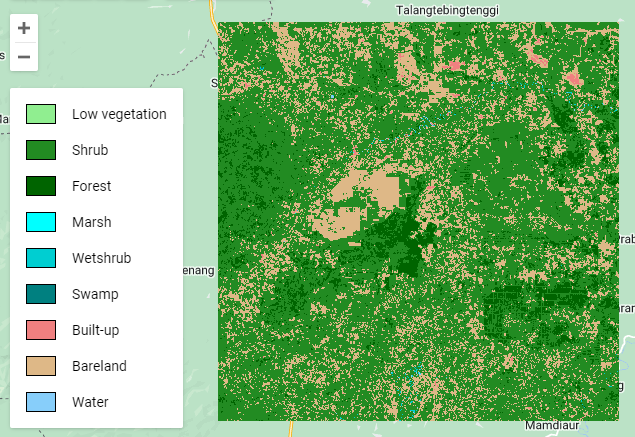
\includegraphics[width=80ex]{lcIndex.png}
	\caption{Land cover from spectral index}
\end{figure}

\section{Vegetation Classification using Machine Learning}
Using spectral indices range to classify land cover or vegetation types is limited. There are more vegetatip type that cant be easily classify such as palm oil, cropland, plantation forest, etc.. There in need more complex classificatio system such as using machine learning.

Machine learning is a term used to describe a complex statistical algorithms which receive inputs or predictors and output a label/value or prediction. Linear regression is machine learning, although most people will likely considered newest and robust one such as decision trees, random forest, support vector machine, and deep learning.

We can utilize some of this machine learning model to help us classify vegetation in Google Earth Engine. All of the machine learning model for either classification and regression can be accessed from \verb|ee.Classifier| class. Some of the model that available are \verb|smileRandomForest, smileGradientTreeBoost, KNN, minimumDistance, & libsvm|. The SMILE part in the class is Statistical Machine Intelligence and Learning Engine, a library of machine learning in Scale, Java, and Kotlin.

To use the model, we need to sample the different type of vegetation and other land cover first. You could do this in GIS program such as QGIS or ArcGIS or you can do it directly in GEE using the drawing features. In GEE, each class should be presented using value of integer: 1, 2, 3, ... So not as a string, where each value represent one class. So when making the geometry as sample as shapefile, the are column with value in integer.

The sample for land cover needed to split into training and testing to see the accuracy of the model. Usually its done by splitting sample for each classes by 4:1 ratio where 4 is for training. After split. You could extract the pixel value from the image using \verb|sampleRegions| method from the \verb|ee.Image| of features to be extracted where the arguments for the collection is the sample. Next the model will be train using the sample where the trained or fitted model will be applied to the image resulting in land cover of vegetation cover. The example of the script used can be seen in Script \ref{code:machineLearning}. Where it utilize \verb|ee.Classifier.smileRandomForest| as machine learning model.

\begin{lstlisting}[language=JavaScript, label={code:machineLearning}, caption={GEE Script to Classify Vegetation Type using Machine Learning}]
// image is the multispectral imagery
// sample is vegetation type or land cover sample

// Column of the class value in integer
var classProperty = 'classvalue'

// Classlist
var values = [1, 2, 3, 4, 5, 6, 7, 8, 9, 10, 11];
var names = ['Grassland', 'Cropland', 'Shrub', 'Palm oil', 'Plantation forest', 'Natural forest', 'Wetland', 'Ricefield', 'Built-up', 'Bareland', 'Water'];
var palette = ['90EE90', 'FFD700', '808000', 'FF4500', 'A0522D', '006400', '40E0D0', '008080', 'F08080', 'DEB887', '87CEFA'];

// Split the sample into train and test
sample = ee.FeatureCollection(values.map(function(value){
	var samplePerClass = sample.filter(ee.Filter.eq(classProperty, value)).randomColumn(); // Add random value column to the sample

	var train = samplePerClass.filter(ee.Filter.lte('random', 0.8)).map(function(feat){ return feat.set('sample', 'train')});

	var test = samplePerClass.filter(ee.Filter.gt('random', 0.8)).map(function(feat){ return feat.set('sample', 'test')});;

	return train.merge(test);
})).flatten();

// Extract value of the image using the sample
var extract = image.sampleRegions({
	collection: sample,
	scale: 30,
	properties: [classProperty, 'sample']
});

// Split it again after extract
var train = extract.filter(ee.Filter.eq('sample', 'train'));
var test = extract.filter(ee.Filter.eq('sample', 'test'));

// Train the model
var model = ee.Classifier.smileRandomForest(50).train(train, classProperty, image.bandNames());

// Classify the image
var lulc = image.classify(model, 'lulc')
	.set({
		lulc_class_values: values,
		lulc_class_palette: palette
	});

// Show the result
Map.addLayer(lulc, {}, 'Land cover');

// Asses the accuracy
var confusionMatrix = test.classify(model, 'prediction').errorMatrix(classProperty, 'prediction');
print('Confusion matrix', cm);
print('Overall accuracy', cm.accuracy());
print('Kappa', cm.kappa());
\end{lstlisting}

\section{Compositing and Preprocessing Multitemporal Satellite Imagery}
To compare the difference between a region between two different time, it is usually common to use multitemporal data. While taking two different data is easy, usually you need to make sure the radiometric value of the same object in different image is the same. It is due to different time might affect the atmospheric condition when the image is taken, usually more cloudy could result in more bright pixel and shadowy could make pixel darker. Other aerial distrubance such as aerosol might affect the valud of the pixel.

To accomodate the variaty of value between two temporal imagery like in different year, it is common to use the same month of at least in the same season. Another technique is using calibrating it using PIF matching or pseudo-invariant feature matching where we pick unchanged pixel between different time then do a linear regression where the label is either the first or the last images. This method expect that it could resulting in more duplicate radiometric between two different temporal image. Script \ref{code:multitemporal} show how to do just that in Earth Engine

\begin{lstlisting}[language=JavaScript, label={code:multitemporal}, caption={GEE Script to Preprocess Multitemporal Image}]
// Importing landsat imagery collection surface reflectance (level 2)
var landsat8 = ee.ImageCollection("LANDSAT/LC08/C02/T1_L2");

// ee.Geometry object to filter and clip image
var roi = ee.Geometry({
	"geodesic": false,
	"type": "Polygon",
	"coordinates": [
		[
			[
				102.72375815056746,
				-3.084684226459141
			],
			[
				103.27307455681746,
				-3.084684226459141
			],
			[
				103.27307455681746,
				-2.5387744837647532
			],
			[
				102.72375815056746,
				-2.5387744837647532
			],
			[
				102.72375815056746,
				-3.084684226459141
			]
		]
	]
});

// Year list to analyze
var years [2021, 2022, 2023];

// Bands list
var bands = ['B1', 'B2', 'B3', 'B4', 'B5', 'B6', 'B7'];

// Image visualization parameter
var vis = { min: [0.1, 0.07, 0.05], max: [0.4, 0.3, 0.2], bands: ['B5', 'B6', 'B7'] };

// Generate image per year
var images = ee.Image(years.map(function(year){

	// Filter the imagery using boundary and date
	var image = landsat8.filterBounds(roi) // Filter by region
		.filterDate(year + '-01-01', year + '-12-31') // Filter by date
		.sort('CLOUD_COVER_LAND') // Sort by the fewest cloud cover
		.first() // Get the first image from the collection
		.clip(roi) // Clip the image
		.select(['SR_B.*'], bands) // Select only useful bands
		.multiply(0.0000275).add(-0.2); // Scaled it to 0-1

	// Show original Image
	Map.addLayer(image, vis, 'Original_' + year);

	return image2022.rename(bands.map(function(band){
		return band + '_' + year;
	})); // Rename band
}));

// Calibration parameter
// Years to calibrate
var yearsCalibrate = [2021, 2022];
var masterYear = 2023;

// Generate sample from the PIF sample generated
// pifSample is the sample for PIF
var extract = images.sampleRegions({
	collection: pifSample,
	scale: 30,
});

// Generate and apply model for each year and bands
var imagesCalibrated = years.map(function(year){
	var calibrated = bands.map(function(band){
		var model = extract.reduceColumns(ee.Reducer.linearFit, [ band + '_' + year, band + '_' + masterYear ]);

		var bandCalibrated = images.select(band + '_' + year).multiply(ee.Number(model.get('scale'))).add(ee.Number(model.get('offset'))).rename(band);
	
		return bandCalibrated;
	});

	// Show calibrated image
	Map.addLayer(calibrated, vis, 'Calibrated' + year);

	return { year: year, image: calibrated };
});
\end{lstlisting}

\section{Applying Vegetation Indices to Multitemporal Data}
If we want to analyze the pattern of vegetation across seasons or year, we can apply vegetation indices to multitemporal imagery. To apply that, we can easily use \verb|map| to the \verb|ee.ImageCollection|. Where on the function we use for looping (map), we can generate vegetation indices. Script \ref{code:multitemporalIndices} show to apply that

\begin{lstlisting}[language=JavaScript, label={code:multitemporalIndices}, caption={GEE Script to Preprocess Multitemporal Image}]
// Importing landsat imagery collection surface reflectance (level 2)
var landsat8 = ee.ImageCollection("LANDSAT/LC08/C02/T1_L2");

// ee.Geometry object to filter and clip image
var roi = ee.Geometry({
	"geodesic": false,
	"type": "Polygon",
	"coordinates": [
		[
			[
				102.72375815056746,
				-3.084684226459141
			],
			[
				103.27307455681746,
				-3.084684226459141
			],
			[
				103.27307455681746,
				-2.5387744837647532
			],
			[
				102.72375815056746,
				-2.5387744837647532
			],
			[
				102.72375815056746,
				-3.084684226459141
			]
		]
	]
});

// Filter images
var images = landsat8.filterBounds(roi).filterDate('2021-01-01', '2023-12-31');

// Function to generate NDVI
function ndvi(image){
	image = image.select(['SR_B.*'], bands) // Select only useful bands
		.multiply(0.0000275).add(-0.2); // Scaled it to 0-1

	// Band map to define the band use for calculation
	var bandMap = {
		NIR: image.select('B5'),
		RED: image.select('B4')
	};

	// Calculate NDVI
	var ndvi = image.expression('NDVI = (NIR - RED) / (NIR + RED)', bandMap);

	return image.select([]).addBands(ndvi);
}

// Apply ndvi function to images
var imagesNDVI = images.map(ndvi);
\end{lstlisting}

\section{Time-series Modelling of Vegetation Indices}
After generating vegetation indices from multiple images, it is not possible to see the pattern. We can observe the pattern by modelling it using chart where we can see the peach and valley of vegetation condition for certain season. We can utilize \verb|ui.Chart| class to plot it. Script \ref{code:timeSeriesModelling} will show you how to do it

\begin{lstlisting}[language=JavaScript, label={code:timeSeriesModelling}, caption={GEE Script for Time Series Modelling}]
// Importing landsat imagery collection surface reflectance (level 2)
var landsat8 = ee.ImageCollection("LANDSAT/LC08/C02/T1_L2");

// ee.Geometry object to filter and clip image
var roi = ee.Geometry({
	"geodesic": false,
	"type": "Polygon",
	"coordinates": [
		[
			[
				102.72375815056746,
				-3.084684226459141
			],
			[
				103.27307455681746,
				-3.084684226459141
			],
			[
				103.27307455681746,
				-2.5387744837647532
			],
			[
				102.72375815056746,
				-2.5387744837647532
			],
			[
				102.72375815056746,
				-3.084684226459141
			]
		]
	]
});

// Filter and apply some function to landsat
var col = landsat8.filterBounds(roi).filterDate('2013-01-01', '2023-12-31').map(function(image){
  // Cloud masking
	var qa = image.select('QA_PIXEL');
  var dilated = 1 << 1;
  var cirrus = 1 << 2;
  var cloud = 1 << 3;
  var shadow = 1 << 4;
  var mask = qa.bitwiseAnd(dilated).eq(0)
    .and(qa.bitwiseAnd(cirrus).eq(0))
    .and(qa.bitwiseAnd(cloud).eq(0))
    .and(qa.bitwiseAnd(shadow).eq(0));

	// Cloud masked image
  var imageChange = image.updateMask(mask).multiply(0.0000275).add(-0.2)
    .select(['SR_B.*'], ['B1', 'B2', 'B3', 'B4', 'B5', 'B6', 'B7']);
  
  // Bandmap
  var bandMap = {
    NIR: imageChange.select('B5'),
    RED: imageChange.select('B4'),
    BLUE: imageChange.select('B2'),
    GREEN: imageChange.select('B3'),
    SWIR1: imageChange.select('B6'),
    SWIR2: imageChange.select('B7')
  };
	// Calculate NDVI
  var ndvi = imageChange.expression('NDVI = (NIR - RED) / (NIR + RED)', bandMap);

  return image.select([]).addBands(ndvi);
});

// Chart to see the pattern
var chart = ui.Chart.image.doySeries(col, roi, ee.Reducer.mean(), 30, ee.Reducer.mean())
  .setChartType('ScatterChart')
  .setOptions({
    dataOpacity: 0.3,
    trendlines: {
			// Show the line model using polynomial
      0: {
        type: 'polynomial',
        opacity: 1,
        color: 'red',
        showR2: true,
        visibleInLegend: true
      }
    }
  });
print(chart);
\end{lstlisting}

The result will be like this Figure \ref{fig:timeSeries}
\begin{figure}[htbp]
	\label{fig:timeSeries}
	\centering
	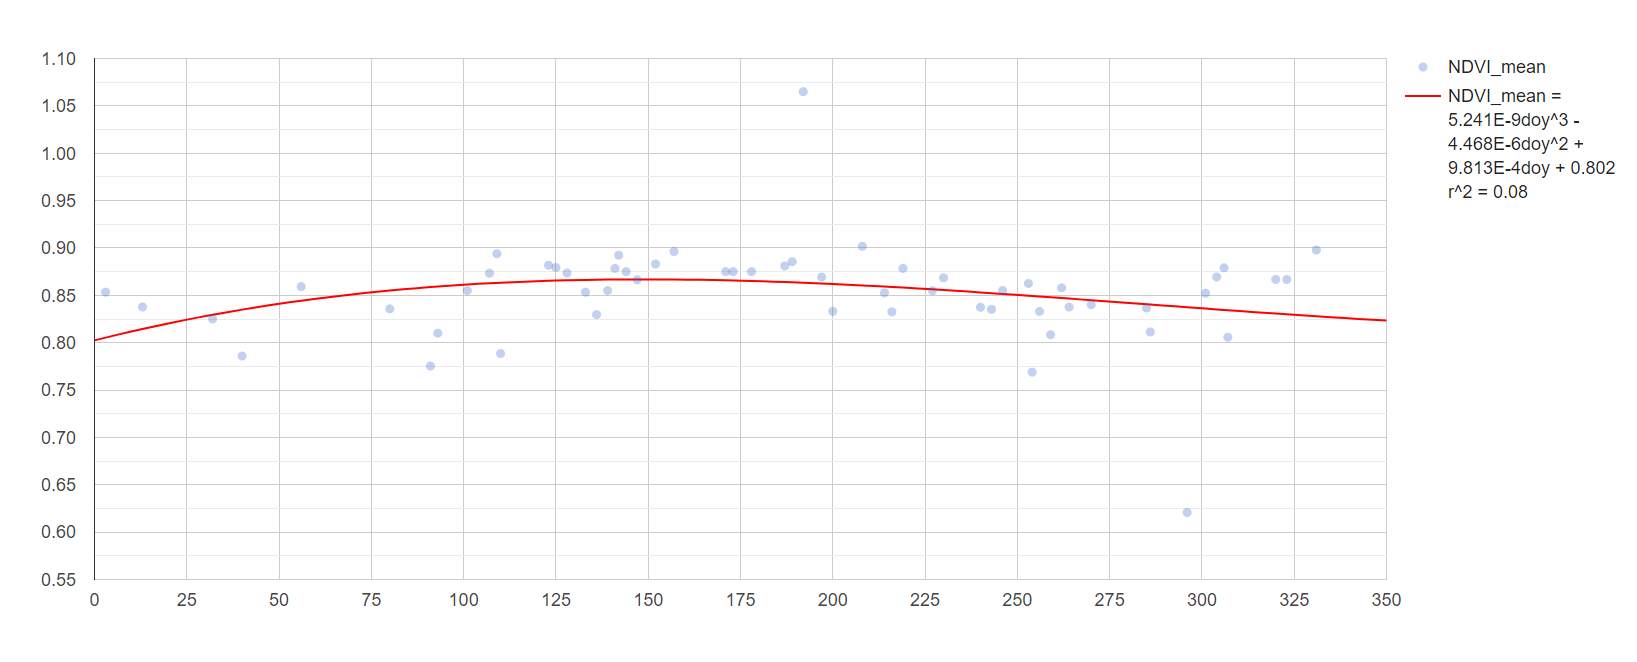
\includegraphics[width=80ex]{timeSeries.png}
	\label{Time series chart of NDVI in region of interest where the horizontal axis represent day in year and vertical axis represent the NDVI}
\end{figure}

\section{Time-series Animation of Vegetation Indices}
While the chart model can be helpful, it is also possible to model it using visualization such as time-series animation. We can utilize \verb|ui.Chart.Thumbnail| to do that. We are also able to use another packages to add text to the animation. Script \ref{code:timeSeriesAnimation}.

\begin{lstlisting}[language=JavaScript, label={code:timeSeriesAnimation}, caption={GEE Script for Time Series Animation}]
// Importing landsat imagery collection surface reflectance (level 2)
var landsat8 = ee.ImageCollection("LANDSAT/LC08/C02/T1_L2");

// ee.Geometry object to filter and clip image
var roi = ee.Geometry({
	"geodesic": false,
	"type": "Polygon",
	"coordinates": [
		[
			[
				102.72375815056746,
				-3.084684226459141
			],
			[
				103.27307455681746,
				-3.084684226459141
			],
			[
				103.27307455681746,
				-2.5387744837647532
			],
			[
				102.72375815056746,
				-2.5387744837647532
			],
			[
				102.72375815056746,
				-3.084684226459141
			]
		]
	]
});

// Add text to image collection
var imageText = landsat8.filterBounds(roi).filterDate('2021-01-01', '2021-12-31').map(function(image){
	var centroid = ee.Geometry.Point(ee.List(roi.centroid(1).buffer(20000).bounds().coordinates().get(0)).get(4));
	
	var label = draw(image.date().format('YYYY-MMMM-dd'), centroid, 100, { fontSize: 32 });
	
	var ndviVisualize = image.visualize({ min: -1, max: 1, palette: ['blue', 'white', 'green'] }).blend(label);
	
	return image.select([]).addBands(ndviVisualize);
});

// Show the GIF
imageText.getVideoThumbURL({
	framesPerSecond: 5,
	dimensions: 480,
	region: roi,
}, function(url, err){
	err ? print(err) : print(url);
});
\end{lstlisting}

\printbibliography